\documentclass{article}

%%% Fill details here (in the second brackets)
\newcommand{\name}{Sam Teeter}     % Your name (First Last)
\newcommand{\wustlkey}{teeters}             % Your WUSTL Key
%%%



%%%%%%%%%%%%%%%%%%%%%% Formatting Stuff %%%%%%%%%%%%%%%%%%%%%%%%%%%
\usepackage{times}
\usepackage[T1]{fontenc}

\setlength{\parskip}{1em}\setlength{\parindent}{0pt}
\linespread{1.25}
\usepackage[margin=0.7in,top=1in]{geometry}\usepackage{fancyhdr}
\pagestyle{fancy}\lhead{\bf \name}\rhead{\bf \wustlkey}\cfoot{\thepage}
\newcommand{\info}{\clearpage \subsection*{Information}}
\newcommand{\solution}[1]{\clearpage \subsection*{Solution #1}}
\newcommand{\spart}[1]{\paragraph{(#1)}}
%%%%%%%%%%%%%%%%%%%%%%%%%%%%%%%%%%%%%%%%%%%%%%%%%%%%%%%%%%%%%%%%%%%


%%% Add any more packages if you want to
\usepackage{amsmath,graphicx}


\begin{document}
%%%%% Main Body goes here

\solution{1}

\spart{a} There are $\binom{N-J}{K}$ ways to choose $K$ inliers, and $\binom{N}{K}$ ways to choose $K$ correspondences total, so the probability of getting $K$ inliers is
\begin{align}
\frac{\binom{N-J}{K}}{\binom{N}{K}}
\end{align}

\spart{b} Since we know the probability of getting a set of $K$ correspondences with no outliers, the probability of at least 1 outlier is
\begin{equation}
1 - \frac{\binom{N-J}{K}}{\binom{N}{K}}
\end{equation}
The probability of getting at least one outlier in every draw of $M$ draws is therefore
\begin{equation}
\left(1-\frac{\binom{N-J}{K}}{\binom{N}{K}} \right)^M
\end{equation}
and the probability that this doesn't happen (i.e., that we get at least one draw with no outliers), is 
\begin{equation}
P = 1-\left(1-\frac{\binom{N-J}{K}}{\binom{N}{K}} \right)^M
\end{equation}
To find the right number of draws for a fixed probability $P$, we just solve for $M$:
\begin{equation}
M = \frac{ \ln(1-P) }{ \ln\left(1-\frac{\binom{N-J}{K}}{\binom{N}{K}} \right) }
\end{equation}

\spart{c} There should be $\binom{I_1}{K}$ unordered sets of $K$ correspondences all belonging to $I_1$ and $\binom{I_2}{K}$ possible sets of $K$ all belonging to $I_2$. (Since these are non-overlapping sets, we don't need to worry about overcounting the intersection). The probability of getting a set of $K$ samples all from one set or the other is therefore
\begin{equation}
\frac{ \binom{I_1}{K} + \binom{I_2}{K} }{ \binom{N}{K} }
\end{equation}

\solution{3}

\spart{a} Consider the equation for the projection coordinates in camera 1:
\begin{equation}
p_1 = 
\begin{bmatrix}
a \\ b \\ c
\end{bmatrix}
=  
\begin{bmatrix}
f_1 & 0 & W/2 & 0 \\
0 & f_1 & H/2 & 0 \\
0 & 0 & 1 & 0
\end{bmatrix}
\begin{bmatrix}
\alpha x' \\ \alpha y' \\ \alpha z' \\ \alpha
\end{bmatrix}
\end{equation}
\begin{align}
x_1 &= \frac{a}{c} = f_1\frac{x'}{z'} + \frac{w}{2} \\
y_1 &= \frac{b}{c} = f_1\frac{y'}{z'} + \frac{H}{2}
\end{align}
Representing $x_1$ and $y_1$ as a vector, we can write
\begin{equation}
\begin{bmatrix}
x_1 \\ y_1 
\end{bmatrix}
= \frac{f_1}{z'}
\begin{bmatrix}
x' \\ y'
\end{bmatrix}
+
\begin{bmatrix}
W/2 \\ H/2
\end{bmatrix}
\end{equation}
If we solve this expression for $\begin{bmatrix} x' \\ y' \end{bmatrix}$ and plug the results into the same formula for camera 2, we get
\begin{equation}
\begin{bmatrix} x_2 \\ y_2 \end{bmatrix}
= \frac{f_2}{z'} \left( \frac{z'}{f_1} \left(
\begin{bmatrix} x_1 \\ y_1 \end{bmatrix}
-
\begin{bmatrix} W/2 \\ H/2 \end{bmatrix}
\right) \right) +
\begin{bmatrix} W/2 \\ H/2 \end{bmatrix}
\end{equation}

\spart{b} As the hint suggests, suppose that all points in our image exist in a plane defined by $z=0$. The projected coordinates for a camera then take the form:
\begin{align}
p &= [K|0]
\begin{bmatrix}
R & t \\
0 & 1 \\
\end{bmatrix}
p' \\
&= 
\begin{bmatrix}
f & 0 & W/2 & 0 \\
0 & f & H/2 & 0 \\
0 & 0 & 1 & 0
\end{bmatrix}
\begin{bmatrix}
R_1 & R_2 & R_3 & t_1 \\
R_4 & R_5 & R_6 & t_2 \\
R_7 & R_8 & R_9 & t_3 \\
0 & 0 & 0 & 1
\end{bmatrix}
\begin{bmatrix}
\alpha x' \\
\alpha y' \\
0 \\
\alpha
\end{bmatrix} \\
&=
\begin{bmatrix}
f \alpha (R_1x' + R_2y' + t_1) + \frac{W}{2}(R_7x' + R_8y' + t_3) \\
f \alpha (R_4x'+R_5y'+t_2) + \frac{H/2}\alpha (R_7x' + R_8y' + t_3) \\
\alpha (R_7x' + R_8y' + t_3)
\end{bmatrix}
\end{align}
The important point here is that by setting $z=0$, we can express the above coordinates in terms of $x', y',$ and $\alpha$. The projection in each camera is therefore a linear transform on the 2d homogeneous coordinates of the point, which we can calculate using an invertible 3x3 transform matrix:
\begin{align}
p_1 &= \begin{bmatrix}
\alpha x'(f_1R_1+W/2R_2) + \alpha y'(f_1R_2+W/2R_8)+\alpha(f_1t_1+W/2t_3) \\
\alpha x'(f_1R_4+H/2R_2) + \alpha y'(f_1R_5+H/2R_8)+\alpha(f_1t_2+H/2t_3) \\
\alpha x'R_7 + \alpha y'R_8 + \alpha t_3
\end{bmatrix} \\
&= \begin{bmatrix}
(f_1R_1+W/2R_2) & (f_1R_2+W/2R_8) & (f_1t_1+W/2t_3) \\
(f_1R_4+H/2R_2) & (f_1R_5+H/2R_8) & (f_1t_2+H/2t_3) \\
R_7 & R_8 & t_3
\end{bmatrix}
\begin{bmatrix}
\alpha x' \\
\alpha y' \\
\alpha 
\end{bmatrix} \\
&= P^{(1)}_{2d}p_{2d}'
\end{align}
To convert from one camera's coordinates to the other, we just need to invert the transformation matrix for the one camera and multiply by the other:
\begin{equation}
p_2 = P^{(2d)}p_{2d} = P^{(2)}_{2d}P^{(1)-1}_{2d}p_1
\end{equation}

\solution{4}

Here is my spliced image for part (b).

\begin{figure*}[!h]
  \centering
  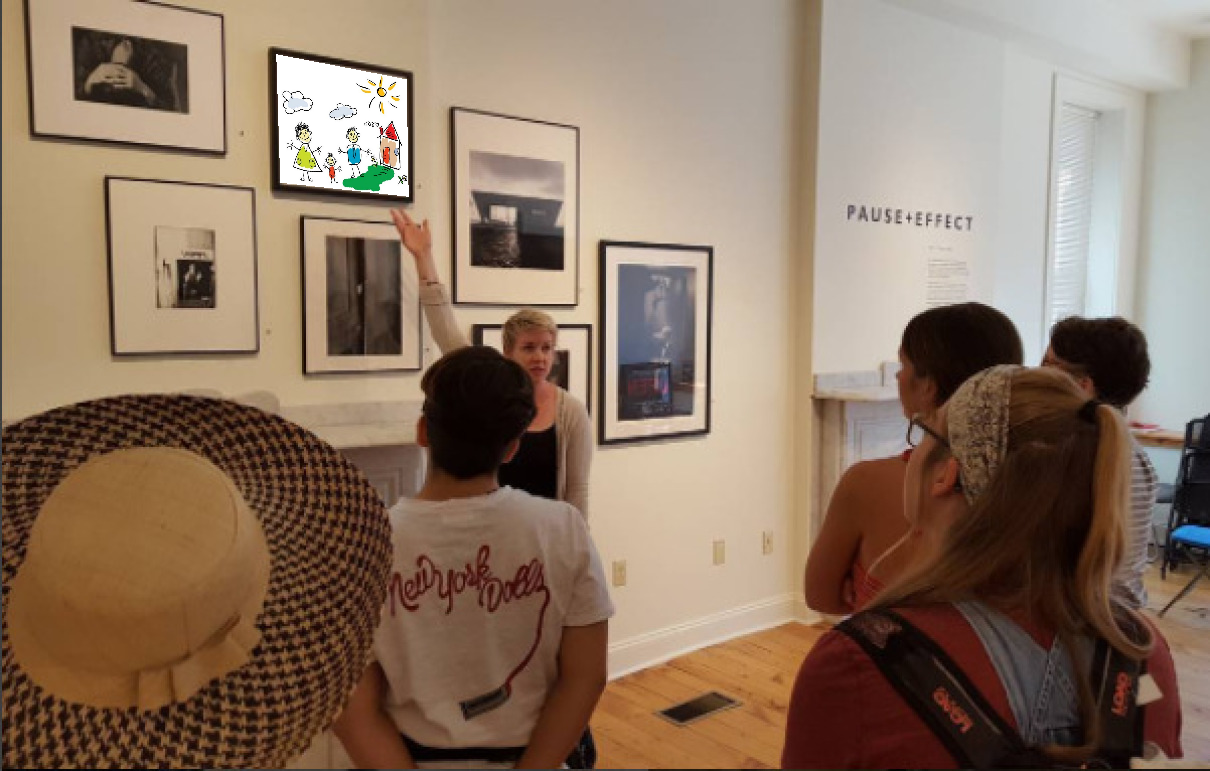
\includegraphics[height=20em]{code/outputs/prob4.png}
  \caption{prob4.png}
\end{figure*}

\solution{5}

Disparity map for part (b).

\begin{figure*}[!h]
  \centering
  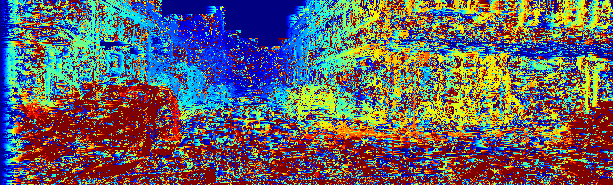
\includegraphics[width=\textwidth]{code/outputs/prob5.png}
  \caption{prob5.png}
\end{figure*}

\info

This problem set took approximately 24 hours of effort.

% Note that you might have to escape some special symbols in URLS like \_
I also got hints from the following sources:
\begin{itemize}
\item Various articles on problem-solving with numpy at stackoverflow.com
\item Numpy documentation
\end{itemize}

\end{document}
\grid
